\chapter{Introduction}\label{chap:introduction}

\section{Motivation}\label{sec:motivation}

The amount of information produced and processed in the world has seen a steady increase over the past decades.
The world internet traffic is increasing exponentially since a few decades.
Edholm's Law\cite{Edholm04} predicts that this behaviour should continue until at least 2030.
It shows that telecommunications data rates are rising in a manner analogous to the one predicted by Moore's Law\cite{Moore98}: doubling every $18$ months.
Even 20 years after this prediction was done, it is still used by organizations responsible by developing the infrastructure to transmit huge amount of data \cite{Mammela17}.

As the amount of data generated by users all around the world increases, the need to store and access this data increases accordingly.
This evolution is matched by an expansion on the number of digital services offered to users: musics, videos, books and other types of files and media that can be accessed from anywhere.
The solution companies found to these problems was Cloud Computing.
Even though Cloud Computing is a vague term, one way to define it is "a technique where IT services are provided by massive low-cost computing units connected by IP networks"\cite{Qian09}.

However, even though Cloud Computing is sold as a way for users to access computing resources they don't have physical access to, the hardware responsible for this computing power must be placed somewhere.
This is achieved by the establishment of multiple data centers all around the world to which devices from anywhere can connect in order to get access to the desired services.
Microsoft, for example, has 300 data centers worldwide to provide their services to their clients\cite{MicrosoftDataCenters}.

A data center is a complex installation that consists of thousands of hard drives connect by kilometers of optical fiber cables.
Therefore, there are massive amounts of investment done in order to create and maintain these facilities.
Microsoft is investing \$80 billion in order to improve their data centers\cite{MicrosoftDataCenters}.
So there is a demand for services related to the maintenance and improvement of data centers.

In this context, one of the main aspects of Cloud Computing in general is the strong virtualization and reliability of the system\cite{Qian09}, meaning that even if some of the hardware fails the service should still be provided without interruption.
So, as hardware components fail, they need to be replaced to ensure that the system keeps working for a long time.

Moreover, in order to maintain a reliable system it is not enough to only replace the hardware after it fails.
In order to prevent some serious issues such as data loss without having to permanently have a copy of all the data it is necessary to predict the hardware failures.

Therefore, one of the main problems faced by data centers is the need to detect which pieces of hardware are going to fail before a fatal crash occurs to allow it to be replaced.
This allows both the prevention of data loss.

Out of all the components that are part of a computer, $80\%$ of the failures occur due to the problems on the hard drives, as indicated by Table \ref{devicefailuretable}
Therefore, there is a special focus on predicting failures on disks.

\begin{table}
    \begin{center}
      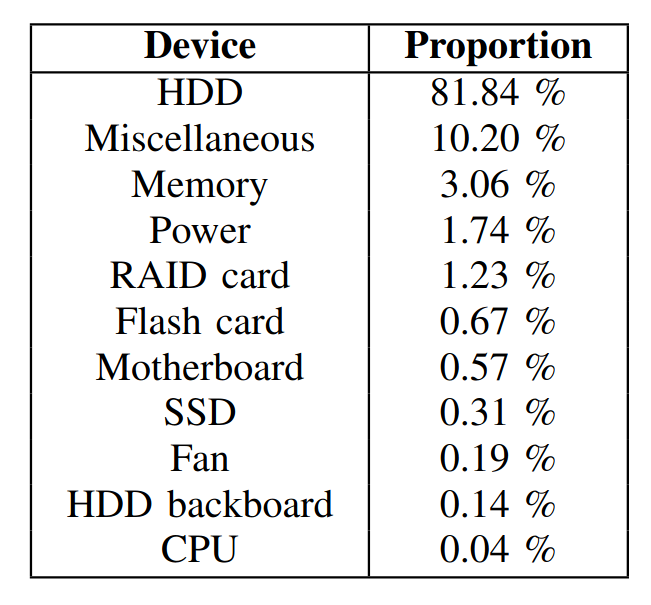
\includegraphics[width=.6\linewidth]{images/FailureProportions.png}
      \caption[Failure percentage by component]{Data center failure percentage by component - \cite{Wang17}}
      \label{devicefailuretable}
    \end{center}
  \end{table}

Hardware vendors are well aware of this situation and the difficulties related to managing thousands of hard drives.
So, in order to allow their users to better tackle these problems, they added a monitoring system to their drives.
This technology is called SMART (Self-Monitoring, Analysis, and Reporting Technology).

Using this protocol, vendors can provide to users indicators of the disk status to the user.
Some of these attributes are Power-On Hours, Air Flow Temperature and Reallocated Sector Count (number of sectors that had to be copied elsewhere on the disk after a failed read or write operation in order to prevent data loss)\cite{SamsungSSD}.

The SMART system can also include status of different attributes.
However, these are limited to threshold not exceeded or threshold exceeded for each attribute, where the threshold is a reference value set by the vendor\cite{SamsungSSD}.

Moreover, even when there is an indication that a threshold has been exceeded, it does not mean that the drive will suffer an unrecoverable failure.
Sometimes it can be a sign that the drive will work more slowly than its specifications indicate.

In addition to that, these status provided by the vendors consider each attribute independently.
They do not take into account the fact that some problems in the hard drive can cause different indicators to increase simultaneously, so by considering the relationship between different attributes would allow problems to be more accurately detected.
For example, having a huge number of Power-On cycles when compared to Power-On hours may indicate a problem in the disk that causes it to crash and restart constantly.

Finally, this ad-hoc approach uses static values and do not consider the evolution of the attributes over time.
Imagine the situation of a disk that has not reallocated any disks so far, and suddenly rate at which sectors have to be reallocated increases.
By taking into account how this attribute evolves over time, this problem can be more quickly detected before the threshold value is reached.

However, even though the built-in failure detection system is not very effective, it doesn't mean that the data itself cannot be used to obtain more interesting results, after all the problem of failure detection must still be solved.
Current research uses mostly machine learning approaches such as SVMs and Neural Networks to tackle this problem.
Further details of how these methods work will be detailed in \hyperref[chap:background]{Chapter 2}. 
% TODO: give a link to the chapter about the current research

This project has three main objectives.
The first one is to create a library that implement some of the current approaches used in research.
The idea is to also made it in such a way that it can be extended with new methods in order to allow them to be easily tested and compared to other ones. 

After creating the library, further tests can be performed on existing methods to understand how they evolve as their parameters change.
For example, the research of Zhu et al. on backpropagation neural networks for disk failure\cite{Zhu13} uses a neural network with one single hidden layer with a fixed amount of 30 nodes on it.
With our library, we can change the number of nodes of a neural network analogous to the one presented by them and study how the results change when the number of layer or nodes is altered.

The third objective is to extend existing methods to also make use of the concept of Health Status introduced by Xu et al.\cite{Xu16}.
Their idea is to give a score from $1$ to $n$ to each sample depending on how close it is to a failure, instead of using only a pass/fail status.

So, the goal is to extend other methods to support more than two classes and study their reaction to this change.
Different models can be extended this way, whether they are other neural network based methods such as \cite{Zhu13} or even if they use other approaches such as the Random Forest one presented by Shen et al.\cite{Shen18}.  

\section{Problem}\label{sec:problem}

Let $x_{i,t}$ be the vector in which the $j^{th}$ component designs the measure of the $j^{th}$ SMART attribute for disk $i$ at time $t$.
As input, we also have a value $y_i$ that is either $0$, if this disk has eventually failed or $1$ if, until the end of the observation period, the disk kept working properly.
Also, let the number of different smart attributes be equal to $m$.

Then given a series of vectors with the SMART attributes for an unseen disk, $\hat{x}_t$, we want to output a value $\hat{y}_t$.
Here, $\hat{y}_t$ should be equal to $1$ if the algorithm predicts that the samples $\left(\hat{x}_1\dots\hat{x}_t\right)$ are closer to the samples in the input that did not fail than to the ones that malfunctioned, and $0$ otherwise.

In a real world scenario, if the value $\hat{y}_t$ is equal to $1$, then a warning should be sent to the people responsible for maintaining the data center in order to replace the concerned disk.

This corresponds to a classical classification problem.
The numerical vectors as input and a binary output suggest that machine learning methods such as Classification Trees\cite{Li14}, Support Vector Machines\cite{Zhu13} and Neural Networks\cite{Xu16} are well adapted to tackle this problem.

However, this problem has  a few specific characteristics.
First of all, the samples are not completely independent, since the values $\left(x_{i,1},x_{i,t}\right)$ are a time series that describe the status of disk $i$ through time.
As we will see on Chapter 3, this can be a motivation to use methods such as LSTM (Long Short-Term Memory) networks that can encode and work with time dependencies.
% TODO: put a link to the chapter here

Moreover, even other methods such as Random Forests that can't easily deal with time dependencies can be extended to make use of the time series aspect of the data.
This can be one by appending new components to $x_{i,t}$ corresponding to the value $x_{i,t}[j] - x_{i,t-\delta}[j], j\in\left\{1,\dots,m\right\}$.
In this case, $\delta$ is a constant that allows the algorithm to detect sudden changes in the value of an attribute\cite{Shen18}.

A second point that needs to be mentioned is that the amount of disks in each class is not similar at all.
Since a hard drive has a service life of around 3 to 5 years\cite{Vishwanath10}, and observations are performed for a few weeks, no failure will be observed for most of the disks.
The ratio of failing disks over the total amount is between $0.4\%$ and $1.9\%$\cite{Xu16}.
So, any approach to this problem has to handle this imbalance in the input data.

Thirdly, the meaning of each SMART attribute is not the same for different vendors\cite{SamsungSSD}.
The protocol is standardized, but what it reports is not.
So, an algorithm for failure prediction cannot be trained on data from different vendor disks.
Moreover, in general, it is not a good idea to mix data from different disks on the same dataset, since they can have different failure causes profiles.

Most of the time, this does not pose a problem to the datasets generated by the data centers.
This is due to the fact that, in practice, a data center uses hundreds of copies of the hardware of the same model and has at most a couple of different models.
This allows for the replacement if failing disks do be done in a cheaper and more swiftly manner, since it simplifies stock management.

% TODO: introduce the concept of time in advance
When evaluating an algorithm there are two main metrics that must be taken into account.
The first one is the FDR (Failure Detection Rate).
This is equal to the ratio between the number of disks that are correctly predicted to be failing and the total amount of failing disks.
Its value should be as close to $1$ as possible

The second metric is the FAR (False Alarm Rate).
This is equal to the ratio between the number of disks that are wrongly predicted to be failing and the total amount of disks that do not fail.
Its value should be as close to $0$ as possible.

The challenge is to find algorithms that find an equilibrium between this values.
If it predicts every $\hat{x}_t$ to give an output $\hat{y} = 1$, the FAR will be equal to $0$, but the FDR too.
On the other hand, if it predicts every $\hat{x}_t$ to give an output $\hat{y} = 0$, the FDR will be equal to $1$, but the FDR too.
So, we notice that a trade off must be done between the FDR and the FAR.

It does not mean, however, that both metrics should be treated identically.
Suppose that during a period of one month, $2\%$ of the hard drives in a data center fail.
This corresponds to a lifetime of about 4 years, which may represent a real world scenario.
If the FDR decreases by $1\%$, then only $0.02\%$ of the disks of the data center will fail without a warning during one month.

In contrast, if the FAR increases by the same amount, then $0.98\%$ of the disks of the whole data center will be unnecessarily replaced during the same period.
This is close to $50\%$ of the disks that actually need to be replaced and can incur a substantial cost.
So, most algorithms in the literature prefer to have a bias towards classifying a disk as working rather than failing.

Aditionnaly, it is impossible to reach perfect values for both indicators.
This is due to the fact that hard drives are subject to real world conditions.
For example, a short circuit on a disk may be caused by an electrical surge, but it does not depend on the internal state of the disk and thus cannot be predicted by the approach using SMART attributes.

Some additional steps can be made after executing the machine learning algorithm.
A common one is the use a voting algorithm.
The simplest way this can be done is as follows\cite{Shen18}: each sample $\hat{x}_{t}, t\in\left\{1,\dots,T\right\}$, often including the change rate components, is evaluated independently.
A sequence $\hat{y}_t, \left\{1,\dots,T\right\}$ is obtained.
Then, a fraction $f$ is chosen.
If more than $f\cdot T$ of $\hat{y}_t$ is equal to $0$ then the output of the system is $0$, otherwise it is $1$.

The main advantage of this method is that it allows to easily control the trade off between the FDR and the FAR which can be desired as we have seen above.
It suffices to increase $f$ in order to decrease the FAR at a cost of also decreasing the FDR.
